\documentclass[10pt]{beamer}
\usetheme{Ilmenau}
\usepackage[utf8]{inputenc}

\usepackage{caption}
\usepackage{graphicx}
\usepackage{amsmath}
\usepackage{amssymb}

\title{Mass Spring Damper}
\subtitle{AE 663 Project}
\institute{Indian Institute of Technology Bombay}
\author{M Suriya Kumar}
\date{\today}

\begin{document}

\begin{frame}[plain]
\maketitle
\end{frame}

\begin{frame}
\frametitle{Table of Contents}
\tableofcontents 
\end{frame}

\section{About the system}

\begin{frame}
\frametitle{Spring mass model with linear viscous damping}
\textbf{Linear viscous damping :} Linear damping occurs when a oscillatory variable is damped 
by an influence that opposes changes in it, in direct proportion to the instantaneous rate of change 
of the variable itself.

\begin{figure}[h]
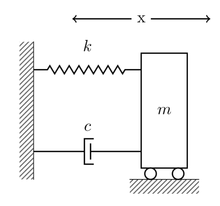
\includegraphics[scale=0.5]{spring_mass_damper.png}
\caption{Mass attached to a spring and damper}
\centering
\end{figure}

Mass($m$) is attached to a Hook's law spring and linear viscous damper. Say the spring constant 
is $k$ and damping coefficient of the damper is $c$.
\end{frame}

\begin{frame}
\frametitle{Deriving equation of motion}
From Newton's law, 
\begin{eqnarray*}
\sum f_{ext} &=& ma, \\
\sum f_{ext} &=& f_s + f_d, \\
f_s &=& -kx, 	\\
f_d &=& -c\dot{x}, \\
-kx - c\dot{x} &=& ma, \\
ma + c\dot{x} + kx &=& 0, \\
m\ddot{x} + c\dot{x} + kx &=& 0
\end{eqnarray*}

Therefore the equation of motion is given by :
\begin{equation}
m\frac{d^2x}{dt^2} + c\frac{dx}{dt} + kx = 0
\label{eom}
\end{equation}
\end{frame}


\section{Mass spring damper as generalized second order system}

\begin{frame}
\frametitle{Second order system}
General second-order system is given by :
\begin{equation}
\ddot{x} + 2\zeta\omega_0\dot{x} + \omega_0^2x = 0
\label{sec_ord_system}
\end{equation}

From \ref{eom} we can get,
\begin{equation}
\ddot{x} + \frac{c}{m}\dot{x} + \frac{k}{m}x = 0
\label{mass_spring_system}
\end{equation}

Comparing coefficient with \ref{sec_ord_system}, we get
\begin{eqnarray}
\zeta &=& \frac{c}{2\sqrt{km}}, \\
\label{def_zeta}
\omega &=& \sqrt{\frac{k}{m}}
\label{def_omega}
\end{eqnarray}

\end{frame}
 
\end{document}

